%\VignetteIndexEntry{Statistical Working Paper on Imputation Methodology for the FAOSTAT Production Domain}
%\VignetteEngine{knitr::knitr}
\documentclass[nojss]{jss}
\usepackage{url}
\usepackage[sc]{mathpazo}
\usepackage{geometry}
\geometry{verbose,tmargin=2.5cm,bmargin=2.5cm,lmargin=2.5cm,rmargin=2.5cm}
\setcounter{secnumdepth}{2}
\setcounter{tocdepth}{2}
\usepackage{breakurl}
\usepackage{hyperref}
\usepackage[ruled, vlined]{algorithm2e}
\usepackage{mathtools}

\usepackage{float}
\usepackage{placeins}
\usepackage{mathrsfs}
\usepackage{multirow}
%% \usepackage{mathbbm}
\DeclareMathOperator{\sgn}{sgn}
\DeclareMathOperator*{\argmax}{\arg\!\max}

\title{Statistical Working Paper on Imputation Methodology for
  the FAOSTAT Production Domain }

\author{Joshua M. Browning, Michael C. J. Kao, Francesca Rosa\\ Food and Agriculture Organization \\ of the United Nations}

\Plainauthor{Joshua M. Browning, Michael C. J. Kao, Francesca Rosa}

\Plaintitle{Statistical Working Paper on Imputation Methodology for
  the FAOSTAT Production Domain }

\Shorttitle{Imputation method}

\Abstract{

 This paper proposes a new imputation method for the FAOSTAT
  domains based on linear mixed model and ensemble learning.

  The proposal provides a resolution to many of the shortcomings of the
  current approach, and offers a flexible and robust framework to
  incorporate further information to improve performance.

  A detailed account of the methodologies is provided. The linear
  cross-commodity information; meanwhile, the ensemble learning approach
  provides flexiblity and robustness where traditional imputation methods
  of applying a single model may have failed.
  \\

}


\Keywords{Imputation, Linear Mixed Model, Ensemble Learning}
\Plainkeywords{Imputation, Linear Mixed Model, Ensemble Learning}

\Address{
  Francesca Rosa\\
  Economics and Social Statistics Division (ESS)\\
  Economic and Social Development Department (ES)\\
  Food and Agriculture Organization of the United Nations (FAO)\\
  Viale delle Terme di Caracalla 00153 Rome, Italy\\
  E-mail: \email{Francesca.Rosa@fao.org}\\
  URL: \url{https://svn.fao.org/projects/SWS/RModules/faoswsProduction/}
}

\usepackage{Sweave}
\begin{document}
\Sconcordance{concordance:methodologyImputation.tex:methodologyImputation.Rnw:%
1 65 1 1 0 47 1 1 4 18 0 1 3 1 1 1 166 47 1 1 15 1 2 36 1 1 6 1 2 142 1 %
1 4 2 0 2 1 3 0 1 2 22 1 1 3 2 0 2 1 3 0 1 2 9 1 1 3 2 0 2 1 3 0 1 2 11 %
1 1 3 2 0 2 1 3 0 1 2 6 1 1 3 2 0 2 1 3 0 1 2 13 1 1 3 2 0 2 1 3 0 1 2 %
13 1 1 3 2 0 2 1 3 0 1 2 10 1 1 3 2 0 2 1 3 0 1 2 22 1 1 3 2 0 2 1 3 0 %
1 2 5 1 1 3 2 0 2 1 3 0 1 2 6 1 1 2 1 0 1 6 5 0 1 2 4 0 1 2 3 1 1 2 1 0 %
2 1 1 2 1 0 2 1 3 0 1 2 11 1 1 8 7 0 1 2 1 0 1 2 1 0 1 2 1 0 1 2 1 0 1 %
3 2 0 1 1 3 0 1 2 22 1 1 3 2 0 2 1 3 0 1 2 6 1 1 3 2 0 2 1 3 0 1 2 5 1}

\SwaveParseOpstions

\section{Introduction}
Missing values are commonplace in the agricultural production domain,
stemming from non-response in surveys or a lack of capacity by the
reporting entity to provide measurement. Yet a consistent and
non-sparse production domain is of critical importance to FAO and to compute Food Balance
Sheets (FBS). Thus accurate and reliable imputation is essential and a
necessary requisite for continuing work. This paper addresses several
shortcomings of the current work and a new methodology is proposed in
order to resolve these issues and to increase the accuracy of
imputation.\\

The primary objective of imputation is to incorporate all
available and reliable information in order to provide best estimates of
food supply in the SUA/FBS.\\

Presented in table \ref{tab:swsflag} is a description of the existing
flags in the current Statistical Working System (SWS). In this
exercise, estimated and previously imputed data are marked as
either \textbf{E} or \textbf{I} and are the target values to
be imputed.\\

\begin{table}[h!]
  \label{tab:swsflag}
  \caption{Description of the flags in the Statistical Working System}
  \begin{center}
    \begin{tabular}{|c||p{12cm}|}
      \hline
      Flags & Description\\
      \hline
      & Official data reported on FAO Questionnaires from countries\\
      I & Imputed figure\\
      T & Unofficial\\
      M & Not reported by country\\
      E & Expert sources from FAO (including other divisions)\\
      \hline
    \end{tabular}
  \end{center}
\end{table}


The set of values considered reliable enough to be considered \textit{protected} is identified by the \textit{flagValidTable}. The following table reports only those flag combination thare will not be overwritten by the module(\textbf{protected figures}):

\newpage

\begin{Schunk}
\begin{Soutput}
    flagObservationStatus flagMethod Valid Protected
 1:                     E          c  TRUE      TRUE
 2:                     E          f  TRUE      TRUE
 3:                     E          h  TRUE      TRUE
 4:                     I          c  TRUE      TRUE
 5:                     M          -  TRUE      TRUE
 6:                     T          -  TRUE      TRUE
 7:                     T          c  TRUE      TRUE
 8:                     T          h  TRUE      TRUE
 9:                     T          p  TRUE      TRUE
10:                                -  TRUE      TRUE
11:                                c  TRUE      TRUE
12:                                h  TRUE      TRUE
13:                                p  TRUE      TRUE
14:                                q  TRUE      TRUE
\end{Soutput}
\end{Schunk}






\subsection{Yield}

The next graph depicts the yield for \textit{wheat}.\\

From the graph, we can first observe that there is a general
increasing trend in the yield accross almost allcountries .
Similar stories are observed in almost all commodities
that have been studied during the development of the methodology. This
is a result of continuous advancement in both technology and
agricultural practice driven by research \& development. Improved
irrigation provides crop with sufficient and uninterrupted water
source, while tailored compound feed provide the precise nutrient
requirements ensuring the livestocks consume the optimal diet for
growth. Regardless whether these practices are sustainable or
beneficial, there are strong evidence of increased productivity over
time.\\

Nevertheless, just like all available technology such as internet, the
distribution is far from perfect. The adoption of technology depends
on the access which may be hindered by the presence of patents, or
restriction imposed by service providers. Imperfect information and
limit financial resources are also major obstacles for embracing the
new developments, this is particularly true for countries where the
majority of the producers are smallholders or subsistence farming.\\

Furthermore, producers face different constraints and cost. Countries
such as Brazil and Russia which have large amounts of arable land do
not bear the same cost for land acqusition in comparison to small
states such as the Netherlands. The cost translates to different
pressure to improve productivity and yield. Required innovations are
also different for countries: wheat breeding for the development of
drought and disease-resistent varieties were crucial to withold
Australia's dry climate.  \\

Despite the differences among countries branching from various
combination of technological advancement and economic condition, these
factors all contribute towards a positive improvement in productitivity
which can be estimated as an aggregated mixture effect.\\

Forces of nature also play a vital role in the determination of crop
productivity. However, unlike technological advancement, precipitation
and temperature are associated more closely to year-to-year variation.\\


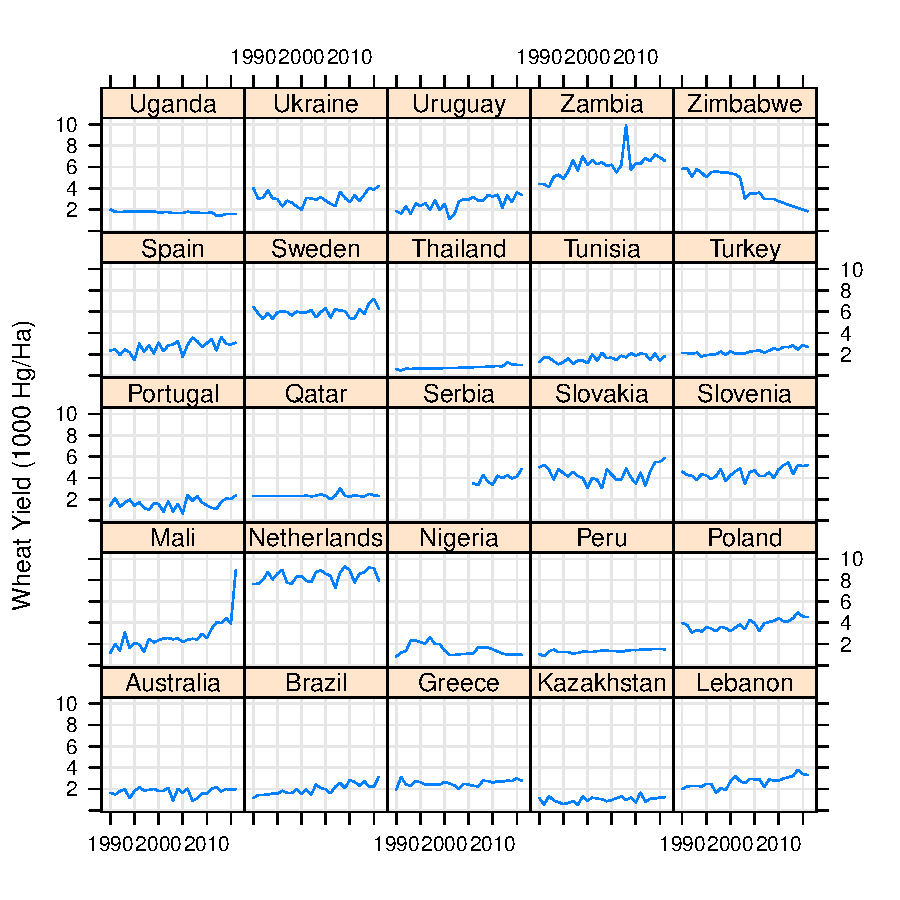
\includegraphics{methodologyImputation-wheat-yield-explore}

\newpage

\FloatBarrier
\subsection{Production and Area Harvested}

Although yield plays a vital role in the production process, the
actual quantity of production is mainly dictated by the area sown and
harvested. The illustration in this section show that the crop-production
series is usually dominated by how much area was planted and
harvested.\\

In contrast to the simple mechanism of yield where all dominant
factors contribute towards improving the productivity, the mechanism
of production is much more unpredictable. \\

Production is determined by area harvested and hence sown in the
previous period by the farmer, which ultimately depends on the
perception of information and subjective judgement of the
producer. Production can increase or decrease  as a response
to the state of the market, where wheat field can be substitue to 
sorghum if prices are expected to be high. Further, individual
entities faces different risk profiles, even under the assumption of
all producers are profit-seeking the risk profile may alter the
portfolio of products held by the producer. Markets have been known to
be difficult to forecast, let alone the prediction of human judgement
is just shy of impossible under curren state of understanding.\\

Only in cases where the commodity is a major staple or exporting item,
we can observe simple trend explained by the continuous increase in
demand. On the other hand, commodities which are of relative lesser
importance, the pattern of the production may display unpredictable
erratic behaviour.\\




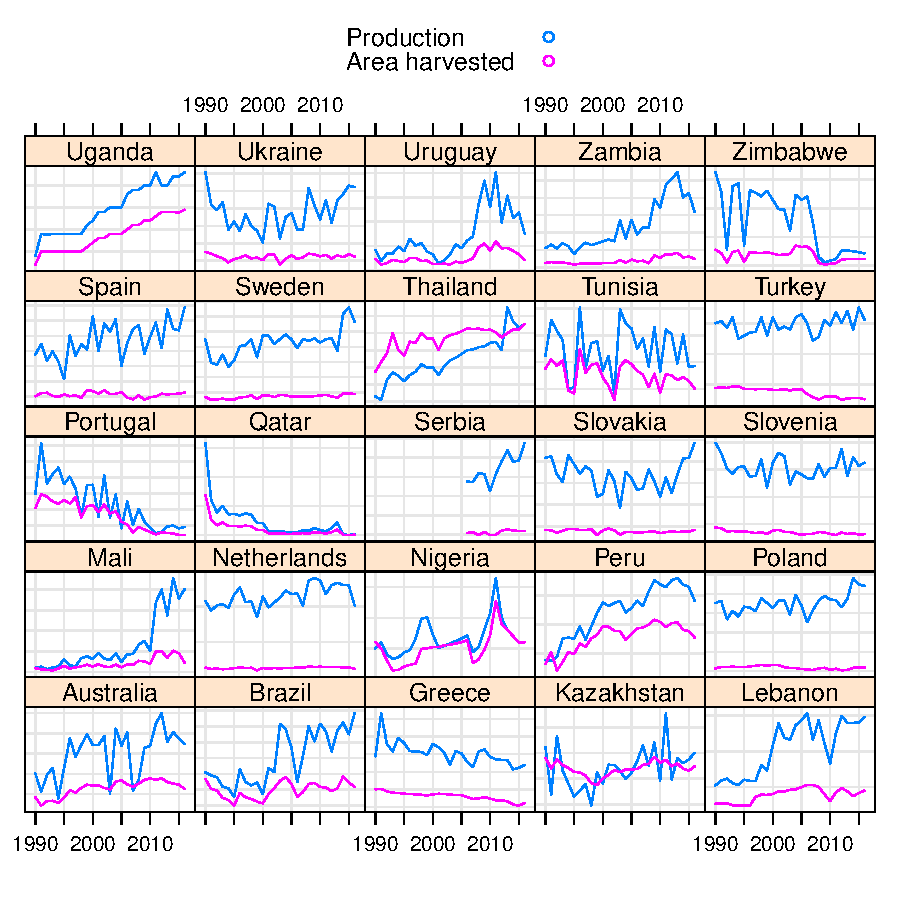
\includegraphics{methodologyImputation-wheat-production-area-explore}


\newpage



\section{Proposed Methodology}

The imputation of missing observations is traditionally done via a model.  For example, we may consider a simple global mean model where we compute the mean of all available observations and use that value to impute missing observations.  Alternatively, we could use a more complex model (i.e. linear/exponential/logistic regression, spline, etc.), fit the model to the available data, and then estimate missing values using this model.  However, this approach has two problems.  First, we may choose a poor model and thus obtain poor estimates.  Second, we have to specify which model to use for each set of data, and this could be very tedious if we have many time-series to impute.  To avoid this problems, we consider ensemble models.

\subsection{Ensemble Imputation}

Ensemble learning refers to the process of building a collection of
simple base models or learners which are later combined to obtain a
composite model or prediction.  One of the most famous applications of ensemble learning was the prediction of movie ratings held by Netflix in which the
top two performers both used an ensemble of different models.  Ensembles are very popular in the data-mining community because of their ability to combine multiple models and come up with an estimate that is better than any of the individual models.\\

The method consist of two steps:
\begin{enumerate}
  \item Building multiple models/learners.
  \item Combining the models or predictions.
\end{enumerate}

The ensemble method reduces the risk of choosing a poor model as we are averaging multiple models.  Thus we reduce the risk of implementing a single model which may produce poor imputations for a certain subset of data. Moreover, model selection is unecessary, since all model are included in the final ensemble.\\

\textit{Thomas Dietterich} describes several problems in machine learning in his paper ``Ensemble Methods in Machine Learning'' (\url{see http://www.eecs.wsu.edu/~holder/courses/CptS570/fall07/papers/Dietterich00.pdf}), and he also discusses how using an ensemble can reduce the errors from the following three issues.

\begin{itemize}
  \setlength{\itemindent}{1in}
  \item[\textbf{Statistical:}] A lack of data may allow multiple models to fit the training set well.
  \item[\textbf{Computational:}] Optimization procedures occasionally converge to local solutions instead of the global solution.
  \item[\textbf{Representational:}] It may not be possible to model the true phenomenon with a known model.
\end{itemize}

\begin{figure}[!ht]
  \centering
  \includegraphics[scale = 0.7]{figure/dietterich.png}
\end{figure}

The \textbf{statistical problem} refers to the lack of data to support a
particular hypothesis. The problem can be formulated as finding the
best hypothesis among competing models in the space
$\mathbf{\mathcal{H}}$. In the top left graph of the
depiction from Dietterich we see a blue boundary, and the idea is that all
models within this boundary will give the same fit to the training data.
Thus, there is insufficient information to determine which one is better.
By combining the models, we reduce the risk of choosing a terrible model.
For example, if we only observe two data points for a country, then
fitting a linear line or a log curve can both give the same accuracy
on the training data and we may have no information to distinguish
between the two.\\

The second problem is that some models are fit by  \textbf{optimizing} some cost function.  These numerical algorithms can often converge to local solutions instead of the global solution.  The top right graph from Dietterich represents this problem, with points h1, h2, and h3 representing the local solutions and f the true global solution.  Thus, combining the multiple fits should get us closer to the true optimum f.  At the time of writing this vignette, no models which use this numerical optimization are present in the default methodology; however, we could introduce such models in the future (for example, a neural network).

The final problem,  \textbf{representational}, refers to the fact that the true
function $f$ can not be represented by any of the individual models. However, by
combining the models we may expand the space of representable
functions and more closely approximate the true function $f$.  For example, if
the production of a country has been growing at a linear rate in the
distant past but has expanded rapidly recently, then neither a linear or
exponential model will provide a satisfactory result. However, an
ensemble combining a linear and exponential model will provide a better
solution by capturing different characteristics of the data.\\

From an implementation point of view, the algorithm is adaptive and will not need constant updating.  For example, If the data generating mechanism changes in the future, the next fit of the ensemble will shift weights to models which better represent the data and thus it will not be necessary to constantly monitor and update the methodologies/models manually.

\subsection{Description of Models}

This section describes the different base learners for the ensemble methodology, and they are listed in increasing order of complexity. An effective ensemble will have base models as diverse as possible. If there is no diversity and all models generate similar results, then little is gained by combining these models and the ensemble model will not be much of an improvement from an individual model.\\

\begin{itemize}
  \item \textbf{Mean}: Mean of all observations
  \item \textbf{Median}: Median of all observations
  \item \textbf{Linear}: Linear Regression
  \item \textbf{Exponential}: Exponential function
  \item \textbf{Logistic}: Logistic function
  \item \textbf{Naive}: Linear interpolation followed by last observation
    carried forward and first observation carried backward.
  \item \textbf{ARIMA}: Autoregressive Integrated Moving Average model
    selected based on the AICC, and imputation via Kalman Filter.
  \item \textbf{LOESS}: Local regression with linear models and model window
    varying based on sample size.
  \item \textbf{Splines}: Cubic spline interpolation.
  \item \textbf{MARS}: Multivariate Adaptive Regression Spline
  \item \textbf{Mixed Model}: Linear mixed model with time as a fixed effect
    and country as the random effect.
\end{itemize}

\subsection{Model ``Level''}

We wish to be able to construct models of varying levels of complexity, and in doing so we would like to be able to build very localized models as well as more general/global models.  One way of doing this is by restricting the training dataset for each model constructed.  For example, if we have fairly good data availability for a particular country/commodity, then we may wish to use only that country's data when building a model.  However, if one country/commodity only has a few valid observations, then we may need to use global trends for that commodity to model that country/commodity more accurately.

In the current code, there are two ``levels'' for constructing a model: ``local'' and ``global.''  The first, ``local,'' means that the model will only use data for that specific slice of data (defined by the byKey parameter) in the fitting of the model.  Thus, we will construct a different model for each different time series slice of the data.  Most of the implemented models fall under this methodology: mean, linear, exponential, logistic, naive, loess, splines, and MARS.

The ``global'' level means that the model uses all the data available.  The mixed model follows this approach in that all data is used to fit a mixed effects model (where year is considered a fixed effect and country a random effect).

\subsection{Extrapolation}

The ensembling process makes use of many different models, but we must be careful in considering what kinds of models to use in which scenarios.  As a simple example, suppose a country has production values of 1, 2, and 4 in three consecutive years and then twenty years of missing data.  If we fit an exponential model to this data, we'll be estimating production values over 4 million at the end of the twenty year period!  In addition, other models (such as splines and LOESS) don't extrapolate well.

Thus, for each model, we have an extrapolation parameter.  This value allows the user to control how far outside the range of the data a particular model can be used.  Using this functionality allows us to prevent extrapolating with models that clearly shouldn't be used outside the range of the data while still making use of these models for interpolation purposes.

\subsection{Computation of Weights}

To construct an ensemble, one has to use a weighted average of all of the input models.  However, one  must determine a meaningful way for computing weights, as models which perform poorly shouldn't receive as much weight as models which fit the data well.  A simple approach is to compare, for each valid observation, the model estimate and the true value.  If we average the error between these two values across all valid observations, we get an estimate for the error of the model.  Then, we can use this error to compute the model weights:

$$w_i = 1/e_i / \sum_{j = 1}^n 1/e_j$$

where $w_i$ is the weight of the $i$th model, $e_i$ is the error of the $i$th model, and $n$ is the total number of models.   Thus, models with smaller errors receive more weight in the final ensemble, and the summation on the bottom of the above formula ensures that the weights sum up to one (ensuring that our weighted sum is in fact a weighted mean).  This approach is possible in the current code by setting the errorType to ``raw'' in the imputation parameters list.

However, the above approach is not ideal.  The problem lies in the fact that complex models generally will fit the training data better because they are more complex.  In reality, we want to know if these models are more accurate at predicting unknown values, and thus we need a way to measure how effectively these models can predict on new observations.  
To accomplish this, one has to use cross-validation.

With cross-validation, the observed data are split into $k$ different groups (often $k=10$, and this is the default for this package as well).  Then, for each group $i$, we build a model using all of the observed data except for those in group $i$ and we measure how well this model estimates the data in group $i$.  If we average this error across all $k$ groups, we get a measure for how well this model predicts on our particular dataset.  We perform this cross-validation error estimation for each of our different models, and then we compute model weights via

$$w_i = \left(1/e_i\right) / \sum_{j = 1}^n \left(1/e_j\right)$$

The formula here is the same as the one above, but now the errors are the average cross-validation errors instead of the errors on the training set.

% \section{Case Studies}
%
% Show a bunch of examples where certain products were imputed.
%
% \section{Simulation Study}
%
% If this is a priority, do a simulation study to show that the method of
% imputation via ensembles is effective.


\section{Models for Ensembling}

This package implements many complex models that may not be familiar to the
user, and so this section goes through the models and describes
how the algorithm works as well as gives an example of the usage of that model.
The order of this section is alphabetical, not by complexity. 
\subsection{defaultArima}

The defaultArima model first fits an AutoRegressive, Integrated Moving Average
(ARIMA) model to the time series provided, and it attempts to find the best
model using the auto.arima function from the \pkg{forecast} package.  If such a
model is found, that model is used (along with KalmanSmooth) to generate
new smoothed estimates of the time series.

\begin{Schunk}
\begin{Sinput}
> model = ensembleModel(model = defaultArima, extrapolationRange = Inf,
+                       level = "local")
> imputationParameters$yieldParams$ensembleModels = list(model)
> imputeVariable(data = exampleData, imputationParameters = imputationParameters)
\end{Sinput}
\end{Schunk}

%' This model often fails, on FAO time-series, and in such cases it is not used in
%' the final ensemble.  Below is an example of when it succeeds, though:
%'
%' <<fig.height=3>>=
%' x = arima.sim(n = 100, model = list(ar = .9))
%' qplot(1:100, x) + geom_line(aes(y = defaultArima(x)))
%' @
%'
%' This example shows one of the common features of the default models: they often
%' set negative values to 0 (as this is the most reasonable thing to do with most
%' of the FAO data).  However, there may be variables where negative values are
%' reasonable, and in such cases an adjusted model should be used.

\subsection{defaultExp}

This algorithm fits the following model: $\log(Y+1) = \beta_0 + \beta_1 t$
where $Y$ is the dependent variable (i.e. production, seed rates, etc) $t$
is time, and $\beta_0, \beta_1$ are the estimated coefficients.  This model is
equivalent to $Y + 1 = e^{\beta_0 + \beta_1 t}$, hence the name exponential.
The 1 in the formula ensures that $\log(Y+1)$ always exists (assuming
$Y \geq 0$).

\begin{Schunk}
\begin{Sinput}
> model = ensembleModel(model = defaultExp, extrapolationRange = 1,
+                       level = "local")
> imputationParameters$yieldParams$ensembleModels = list(model)
> imputeVariable(data = exampleData, imputationParameters = imputationParameters)
\end{Sinput}
\end{Schunk}

\subsection{defaultGlobalMean}

This model is quite simple: it computes the mean from all available
observations and uses that value to impute any missing values.  This model is
not recommended for most domains; however, it may perform reasonably well when
imputing rates or proportions, as the average may not vary drastically from
country to country.  A variable like production is very different, values can
vary drastically in scale and so a global mean is not appropriate.

\begin{Schunk}
\begin{Sinput}
> model = ensembleModel(model = defaultGlobalMean, extrapolationRange = Inf,
+                       level = "global")
> imputationParameters$yieldParams$ensembleModels = list(model)
> imputeVariable(data = exampleData, imputationParameters = imputationParameters)
\end{Sinput}
\end{Schunk}

Note that in the above figure, the imputed values may appear to be different.
However, this is simply due to the different scale in each of the grids; the
imputed value is always about 8.

\subsection{defaultGlobalMedian}

The global median works exactly the same as the global mean, but computes the
median instead of the mean.  Again, this type of model should only be used when
imputing rates or something similar (i.e. no drastic differences in scale
across groups).

\begin{Schunk}
\begin{Sinput}
> model = ensembleModel(model = defaultGlobalMedian, extrapolationRange = Inf,
+                       level = "global")
> imputationParameters$yieldParams$ensembleModels = list(model)
> imputeVariable(data = exampleData, imputationParameters = imputationParameters)
\end{Sinput}
\end{Schunk}

\subsection{defaultLm}

The defaultLm model uses a simple linear regression model for imputation.  It
fits a model of the form: $Y = \beta_0 + \beta_1 t$, where $Y$ is the value to
impute, $t$ is the time, and $\beta_0, \beta_1$ are estimated coefficients.

\begin{Schunk}
\begin{Sinput}
> model = ensembleModel(model = defaultLm, extrapolationRange = Inf,
+                       level = "local")
> imputationParameters$yieldParams$ensembleModels = list(model)
> imputeVariable(data = exampleData, imputationParameters = imputationParameters)
\end{Sinput}
\end{Schunk}

\subsection{defaultLoess}

The defaultLoess model works by fitting a ``local'' linear regression model at
each point in the model space.  The model is local in the sense that the fit at
time $t$ uses only nearby time points, say $t-k$ to $t+k$.  Furthermore, points
further away from $t$ are given less weight in the regression model.  This type
of model has several tuning parameters such as the size of the neighborhood and
the degree of model to fit (i.e. we could fit local linear models, quadratic,
etc.).  For simplicity, we use a local linear model, and we choose the smallest
span possible to allow for the most flexible model.  Addditionally, the local
nature of the loess model means that it likely will not extrapolate well, so
the recommended extrapolation range is 1.

\begin{Schunk}
\begin{Sinput}
> model = ensembleModel(model = defaultLoess, extrapolationRange = 1,
+                       level = "local")
> imputationParameters$ensembleModels = list(model)
> imputeVariable(data = exampleData, imputationParameters = imputationParameters)
\end{Sinput}
\end{Schunk}

\subsection{defaultLogistic}

Logistic curves are S-shaped curves of the form
$$f(x) = A + \frac{B}{1 + e^{-C(t-D)}}$$.
These types of functions make sense in scenarios where a variable is increasing
but may have some upper bound (i.e. production may increase greatly as
technology improves, but there is some maximum production level a country can
obtain).  This algorithm attempts to first fit all four parameters above via
numerical least squares.  If that approach fails, $A$ is assumed to be 0 and
numerical least squares are tried again.  If that model also fails, $B$ is
assumed to be the largest value and model fitting proceeds via generalized
least squares.

\begin{Schunk}
\begin{Sinput}
> model = ensembleModel(model = defaultLogistic, extrapolationRange = 1,
+                       level = "local")
> imputationParameters$ensembleModels = list(model)
> imputeVariable(data = exampleData, imputationParameters = imputationParameters)
\end{Sinput}
\end{Schunk}

Note: in the first example, the logistic regression decays rapidly to 0.  This may not be very reasonable, and thus we recommend using a small extrapolation range for this model.

\subsection{defaultMars}

The defaultMars model uses a technique known as Multivariate Adaptive
Regression Splines (MARS).  This algorithm seeks to model the data using
piecewise linear regression splines, and it determines the breakpoints of the
splines using some optimization criterion.  On our sample dataset, we don't see
anything too interesting:

\begin{Schunk}
\begin{Sinput}
> model = ensembleModel(model = defaultMars, extrapolationRange = Inf,
+                       level = "local")
> imputationParameters$ensembleModels = list(model)
> imputeVariable(data = exampleData, imputationParameters = imputationParameters)
\end{Sinput}
\end{Schunk}

%' To see how this model works, we can instead look at a little toy example.
%' Suppose that our data is constant for the first 10 observations and then
%' increases linearly for the following 10 observations.  And, suppose that we
%' can't measure our data perfectly, but that we have some observation error.
%' The below R code implements such a model, and shows how the MARS approach will
%' fit that data (MARS is named ``earth'' within R because MARS is a proprietary
%' term).
%'
%' <<fig.height=3>>=
%' smallExample = data.table(x = 1:20, y = c(rep(0, 10), 1:10) +
%'                               rnorm(20, sd = .2))
%' fit = earth::earth(y ~ x, data = smallExample)
%' invisible(smallExample[, earthFit := predict(fit)])
%' ggplot(smallExample, aes(x = x, y = y)) + geom_point() +
%'     geom_line(aes(y = earthFit))
%' @

\subsection{defaultMean}

This model computes a mean on each subset of the data and uses that one value to
impute any missing values.

\begin{Schunk}
\begin{Sinput}
> model = ensembleModel(model = defaultMean, extrapolationRange = Inf,
+                       level = "local")
> imputationParameters$ensembleModels = list(model)
> imputeVariable(data = exampleData, imputationParameters = imputationParameters)
\end{Sinput}
\end{Schunk}

\subsection{defaultMedian}

This model computes a median on each subset of the data and uses that one value to
impute any missing values.

\begin{Schunk}
\begin{Sinput}
> model = ensembleModel(model = defaultMedian, extrapolationRange = Inf,
+                       level = "local")
> imputationParameters$ensembleModels = list(model)
> imputeVariable(data = exampleData, imputationParameters = imputationParameters)
\end{Sinput}
\end{Schunk}

\subsection{defaultMixedModel}

The defaultMixedModel is a more complex model that's fit to global datasets
(rather than each individual time-series).  So, let's use a different dataset
to run some analyses with this model:

\begin{Schunk}
\begin{Sinput}
> mixedModelData = extractedData[geographicAreaM49 < 100, ]
> # mixedModelData = processProductionDomain(mixedModelData,
> #         processingParameters = defaultProcessingParameters())
> updateMissingFlags = function(data, value, flag, missingFlag = "M"){
+     missingIndex = which(is.na(data[[value]]))
+     invisible(data[missingIndex, `:=`(c(flag), list(missingFlag))])
+ }
> updateMissingFlags(data = mixedModelData, value = "Value_measuredElement_5421",
+          flag = "flagObservationStatus_measuredElement_5421")
\end{Sinput}
\end{Schunk}

Now, let's run the ensemble imputation with the default imputation parameters.
This example uses the \pkg{lme4} package to fit a mixed model.

\begin{Schunk}
\begin{Sinput}
> newParameters = defaultImputationParameters(5421)
> newParameters$newImputationColumn = "test"
> newParameters$estimateNoData = TRUE
> model = ensembleModel(model = defaultMixedModel, extrapolationRange = Inf,
+                       level = "global")
> newParameters$ensembleModels = list(model)
> imputeVariable(data = mixedModelData, imputationParameters = newParameters)
\end{Sinput}
\end{Schunk}

For most cases, we see the same results as we did with the linear regression: a
simple least-squares curve is fit to the available data and then that model is
used to impute the missing values.  However, the mixed model fit to the data
can also be used for estimation on time-series where very little data is
available, for example on area 46 and 66.

More complex cases are also available: for example, we could fit a hierarchical
model (also with the \pkg{lme4} package) that allows us to impute countries
with missing data based on some hierarchy (for example, continents).  In this
example, we just made up arbitrary regions.

\begin{Schunk}
\begin{Sinput}
> invisible({
+     mixedModelData[geographicAreaM49 == "66", Value_measuredElement_5421 := NA]
+     mixedModelData[geographicAreaM49 == "66",
+                flagObservationStatus_measuredElement_5421 := "M"]
+     mixedModelData[,region := factor(ifelse(geographicAreaM49 < 15, 1,
+                                      ifelse(geographicAreaM49 < 50, 2, 3)))]
+ })
> formals(defaultMixedModel)$modelFormula = Value_measuredElement_5421 ~
+     timePointYears*region + (timePointYears|geographicAreaM49/region)
> hierarchical = ensembleModel(model = defaultMixedModel, level = "global",
+                              extrapolationRange = Inf)
> globalMean = ensembleModel(model = defaultGlobalMean, level = "global",
+                            extrapolationRange = Inf)
> globalMedian = ensembleModel(model = defaultGlobalMedian, level = "global",
+                              extrapolationRange = Inf)
> newParameters$ensembleModels = list(hierarchical = hierarchical,
+                                     globalMean = globalMean,
+                                     globalMedian = globalMedian)
> imputeVariable(data = mixedModelData, imputationParameters = newParameters)
\end{Sinput}
\end{Schunk}

In this complicated example, we can see several different types of imputation
occurring.  The most common case seems to be the hierarchical model, which
simplifies to just a linear regression on countries with enough data to fit
the model.  The global mean and median don't seem to be as good of models, but
in a few cases they provide some value.

Note that we are also able to impute values in region 66, where no data exists
(because we deleted the one value that was present before we began).  This
imputation was performed by looking at the cross-validation error of the three
models considered on all the other datasets and averaging the error across all
available observations.  Generally the mixed model performs best, and so it
gets the most weight on this set of data where we have no available data.

\subsection{defaultNaive}

This model performs simple linear interpolation between available observations.
However, if a missing value is outside the range of the data, then this model
estimates that value by carrying back the first observation or carrying forward
the last observation (depending on if the missing value is before the available
data or after it).  Because of this, this model is not recommended for
extrapolation (and has a default extrapolationRange of 0 in allDefaultModels).

\begin{Schunk}
\begin{Sinput}
> model = ensembleModel(model = defaultNaive, extrapolationRange = 0,
+                       level = "local")
> imputationParameters$ensembleModels = list(model)
> imputeVariable(data = exampleData, imputationParameters = imputationParameters)
\end{Sinput}
\end{Schunk}

\subsection{defaultSpline}

The defaultSpline model uses the spline function from the stats package (part
of base) to fit a spline to the available observations.  Missing observations
are then imputed by the spline estimate at that location.

\begin{Schunk}
\begin{Sinput}
> model = ensembleModel(model = defaultSpline, extrapolationRange = 0,
+                       level = "local")
> imputationParameters$ensembleModels = list(model)
> imputeVariable(data = exampleData, imputationParameters = imputationParameters)
\end{Sinput}
\end{Schunk}


\end{document}



